\section{算法设计与分析}

% \subsection{问题描述}
% 首先基于统计数据,
% 然后建立交通网络的模型,根据模型列出对应的VSP问题方程并求解,以便之后优化问题的求解和模拟,
% 使用SimPy包对不同结果进行模拟。

\subsection{现有交通调度方案分析}
现有运营方案下,校园公交人流量高峰时期常采用多车次连续发车的方法,
由于公交线路站点大多均匀坐落在校园主干道上,高峰时期车辆行进速度也会受到主干道交通环境影响,
导致部分站点排队时间较长;非高峰时期,为考虑运营成本,公交会在始发站待乘客达到一定数量后再发车,
导致在非始发站点等待时间过长,现有的调度策略存在滞后性。通过对客流大数据进行挖掘分析,
运用机器学习算法对客流量模式进行识别,通过该模式建立数学模型,
使用运筹学方法从成本、效益、乘客舒适度等多个角度出发,对公交站定址、
调度策略等特征进行优化,最终解决现有策略下校园公共交通系统中的缺陷。

\subsection{单服务台负指数分布排队系统建模}

在一个由k个串行车站组成的排队系统中,每个车站的服务时间相互独立,服从参数为$k\mu$的负指数分布,
而整个系统的服务时间则服从$k$阶爱尔朗分布。与指数分布相比,爱尔朗分布族具有更大的适应性。
值得注意的是,当k=1时,爱尔朗分布化为负指数分布,并可进一步推导出对于单个车站而言,到达人数近似服从泊松分布,
由于泊松分布的无记忆性\cite{gll},因此更适用于描述排队系统。
\\
\begin{figure}[htbp!]
    \centering
    \subfigure[k=1的爱尔郎分布\label{fig31:sub1}]{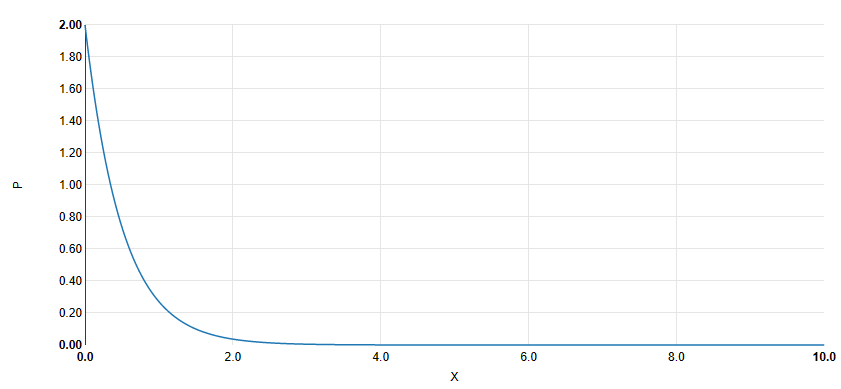
\includegraphics[width=0.3\textwidth]{figs/chap03/elarng.png}}
    \subfigure[泊松分布\label{fig31:sub2}]{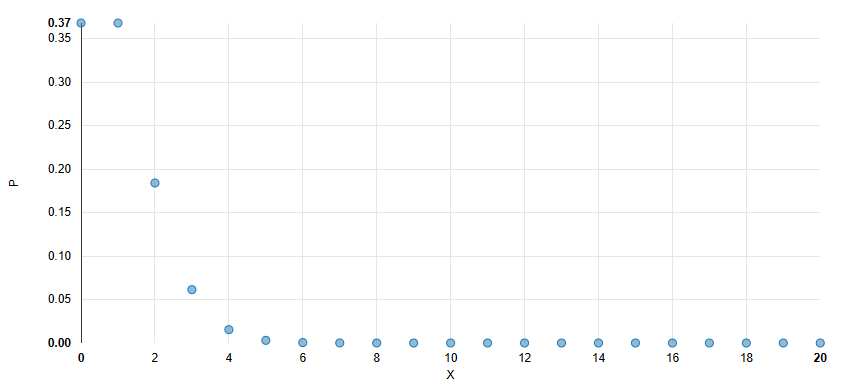
\includegraphics[width=0.3\textwidth]{figs/chap03/possion.png}}
    \caption{两种分布对比图}
    \label{dis1}
\end{figure}

前文给出了单服务台负指数分布排队系统(M/M/1/ $\infty $ / $\infty $)的基本方程~\ref{fomula1}~和状态图~\ref{fig21}~,由图图~\ref{fig21}~
可知,状态 $0$ 转移到状态 $1$ 的转移率为 $\lambda P_0$ ,状态 $1$ 转移到状态 $0$ 的转移率为 $\mu P_1$。由排队系统生灭状态的平衡性质可知,对于状态0必须满足如下方程:
$$\lambda P_0 = \mu P_1$$
对于任意的 $n \ge 1$ 的状态,都可以得到式~\ref{fomula1}~中的方程,求解~\ref{fomula1}~得:
$$P_1 = (\lambda / \mu)P_0$$
易证:
$$P_2 = \left(\lambda / \mu \right)^2 P_0$$
$$……$$
$$P_n = \left(\lambda / \mu \right)^n P_0$$
令 $\rho = \frac{\lambda}{\mu} < 1$,由概率的性质
$$\sum_{n=0}^{\infty}p_n = 1$$ 可以得到站台中乘客数为n的概率 $$P_n = (1-\rho)\rho^n, n \le 1, \rho < 1$$
其中 $\rho$ 代表系统的平均服务率,它刻画了服务机构的繁忙程度;所以又称服务机构的利用率。

由此可以得到一个平均到达率为 $\lambda$,平均服务率 $\mu$ 的排队系统的几个主要指标:

(1)乘客到达后不能及时得到服务需要等待的概率(系统服务强度):
\begin{equation}\label{fomula31}
    P_w = \frac{\lambda}{\mu}
\end{equation}
% $$P_w = \frac{\lambda}{\mu}$$

(2)系统空闲的概率:
\begin{equation}
    P_0 = 1-\frac{\lambda}{\mu}
\end{equation}
% $$P_0 = 1-\frac{\lambda}{\mu}$$

(3)系统中平均乘客长度(队长的期望值)
\begin{equation}
    L_s = \frac{\lambda}{\mu - \lambda}
\end{equation}
% $$L_s = \frac{\lambda}{\mu - \lambda}$$

(4)在队列中等待的平均顾客数(队列长期望值)
\begin{equation}
    L_q = L_s - \rho = \frac{\rho \lambda}{\mu - \lambda}
\end{equation}
% $$L_q = L_s - \rho = \frac{\rho \lambda}{\mu - \lambda}$$

(5)在系统中顾客逗留时间的期望值
\begin{equation}
    W_s = E[W] = \frac{1}{\mu - \lambda}
\end{equation}
% $$W_s = E[W] = \frac{1}{\mu - \lambda}$$

(6)队列中顾客等待时间的期望值
\begin{equation}\label{fomula36}
    W_q = W_s - \frac{1}{\mu} = \frac{\rho}{\mu - \lambda}
\end{equation}
% $$W_q = W_s - \frac{1}{\mu} = \frac{\rho}{\mu - \lambda}$$


% 解决排队问题首先要根据原始资料作出乘客到达间隔和服务时间的经验分布,根据以往经验,校园公交车站客流呈周期性变化,
% 选择文德楼北上行线车站实地统计,该车站位于校门、宿舍楼、主教学楼连接处的枢纽位置,客流量较有代表性,采样地点如图~\ref{fig31}~。
% \\
% \begin{figure}[htbp!]
%     \centering
%     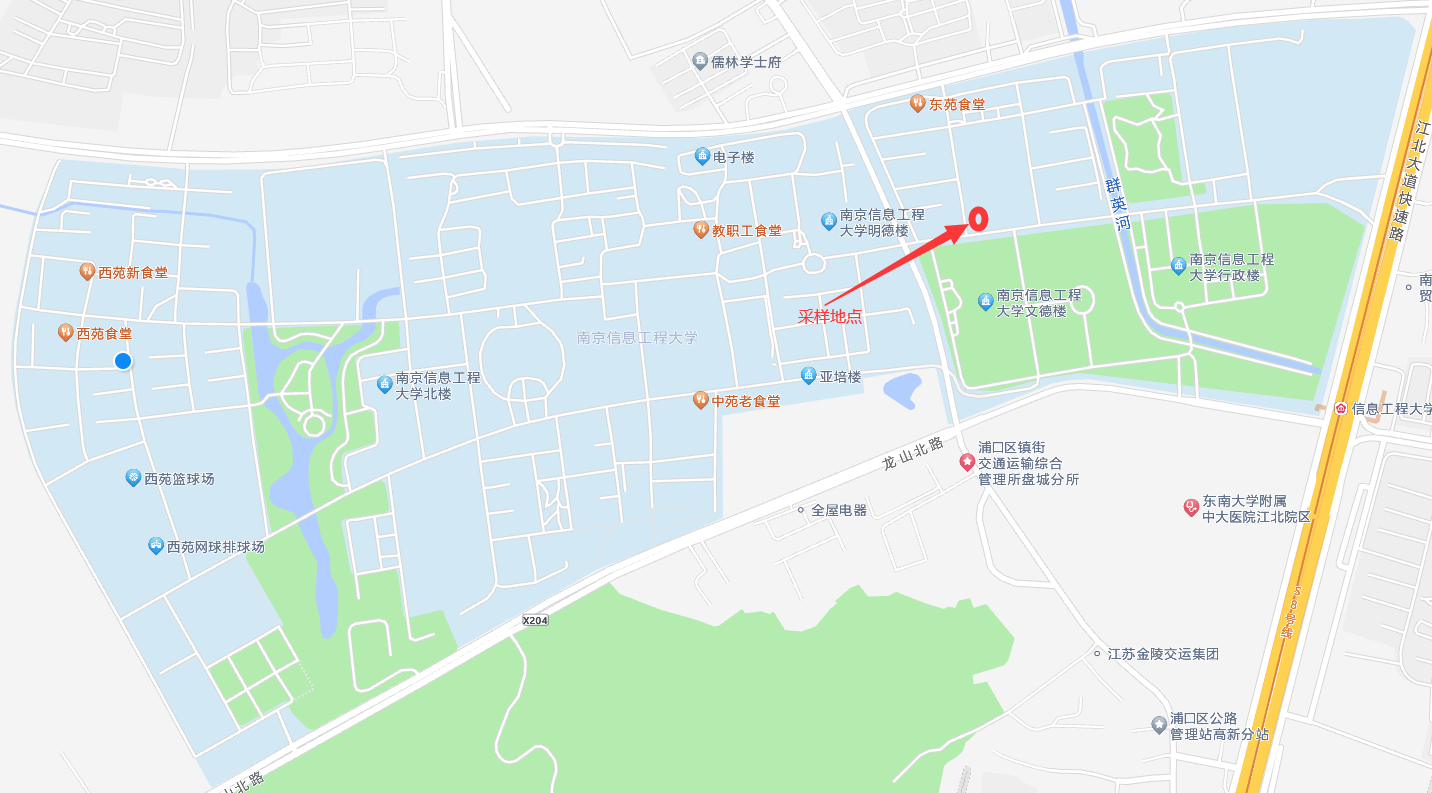
\includegraphics[width=0.95\textwidth]{figs/chap03/map.png}
%     \caption{采样地点}
%     \label{fig31}
% \end{figure}

% 原始数据记载乘客到达时刻和对应的等待时间,以 $\tau_i$ 表示第i个乘客到达的时刻,以s表示等待时间可以得出相继到达时间 $t_i \left(t_i = \tau_{i+1} - \tau_i\right)$ 和等待时间 $w_i$,
% 它们的关系如图~\ref{fig32}~。

% 由图~\ref{fig32}~可以得到如下关系:

% 间隔\quad \quad \quad \quad$t_i = \tau_{i+1} - \tau_i$

% 等待时间 \quad \quad 
% $
% w_{i+1} = 
% \begin{cases}
%     w_i + s_i - t_i,\quad w_i + s_i - t_i > 0
%     \\
%    0, \qquad \qquad \quad w_i + s_i - t_i < 0
% \end{cases}
% $


% \begin{figure}[htbp!]
%     \center
%     \subfigure[$w_i + s_i - t_i > 0$]{\label{queue1}
%     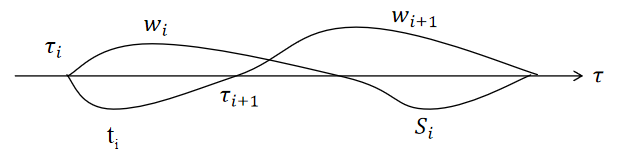
\includegraphics[width=0.6\textwidth]{figs/chap03/queue1.png}
%     }
%     \\
%     \subfigure[$w_i + s_i - t_i < 0$]{\label{queue2}
%     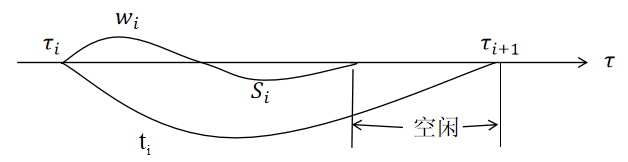
\includegraphics[width=0.6\textwidth]{figs/chap03/queue2.png}
%     }
%     \caption{相继到达的间隔时间和排队等待时间关系示意图}\label{fig32}
% \end{figure}

% 由图~\ref{fig32}~可以得到如下关系:

% 间隔\quad \quad \quad \quad$t_i = \tau_{i+1} - \tau_i$

% 等待时间 \quad \quad 
% $
% w_{i+1} = 
% \begin{cases}
%     w_i + s_i - t_i,\quad w_i + s_i - t_i > 0
%     \\
%    0, \qquad \qquad \quad w_i + s_i - t_i < 0
% \end{cases}
% $



% 以大约两节课的时间(两小时)为一个周期,5分钟为间隔进行采样,将所统计的一个周期内的客流数据
% 经以上关系整理后所得结果如表~\ref{table_1}~所示。
% \begin{table}[htbp!]
%     \centering
%     \caption{车站乘客到达人数分布表}\label{table_1}
    
%     \begin{tabular}{cccc}
%     \whline 
%     时间段 & 到达人数 & 时间段 & 到达人数 \\ 
%     \hline 
%     14:00$ \sim $14:05 & 18 &15:00$ \sim $15:05&5\\ 
%     14:06$ \sim $14:10 & 7 &15:06$ \sim $15:10&2\\ 
%     14:11$ \sim $14:15 & 4 &15:11$ \sim $15:15&3\\ 
%     14:16$ \sim $14:20 & 8 &15:16$ \sim $15:20&6\\ 
%     14:21$ \sim $14:25 & 1 &15:21$ \sim $15:25&5\\ 
%     14:26$ \sim $14:30 & 5 &15:26$ \sim $15:30&67\\ 
%     14:31$ \sim $14:35 & 1 &15:31$ \sim $15:35&8\\ 
%     14:36$ \sim $14:40 & 3 &15:36$ \sim $15:40&12\\ 
%     14:41$ \sim $14:45 & 5 &15:41$ \sim $15:45&8\\ 
%     14:46$ \sim $14:50 & 6 &15:46$ \sim $15:50&3\\ 
%     14:51$ \sim $14:55 & 2 &15:51$ \sim $15:55&4\\ 
%     14:56$ \sim $15:00 & 2 &15:56$ \sim $16:00&2\\ 
%     \whline 
%     \end{tabular}
%     \end{table}

% 统计同时段内车辆到达时间,可以估算出乘客的平均等待时间,如表~\ref{teble_2}~所示。
% \begin{table}[htbp!]
%     \centering
%     \caption{车站平均等待时间表}\label{teble_2}
%     \begin{tabular}{cc}
%         \whline
%         等待时间(分钟) & 频次 \\
%         0 & 23\\
%         1 & 31\\
%         2 & 27\\
%         3 & 25\\
%         4 & 33\\
%         5 & 19\\
%         6 & 22\\
%         7 & 19\\
%         8 & 8\\\
%         >10&0 \\
%         \whline
%     \end{tabular}
% \end{table}

% 由统计结果可以得到公交站这一排队系统的几个特征:

% 平均到达率:$$\lambda \approx 1.56$$ 

% 平均等待时间:4.30(min)

% 平均服务率:$$\mu = 1/4.30 \approx 0.23$$

% 系统的服务强度:$$\rho = \frac{\lambda}{\mu} \approx 6.67 $$

% 因为服务强度大于1,说明系统的服务能力不足以应对到达率,系统会出现排队现象,
% 排队长度可能会不断增加。如果希望系统稳定运行,需要增加服务能力或降低到达率。

使用一个Python类描述系统提供的服务,代码如下:
\begin{lstlisting}[breaklines=true,language=Python]
    class System(object):
        def __init__(self, env, numService, miuService_):
            self.env = env
            self.service = simpy.Resource(env, numService)
            self.miuService = miuService_

        def beingServed(self):
            yield self.env.timeout(random.expovariate(self.miuService))
\end{lstlisting}

通过上述指标对车站客流进行模拟,核心实现代码如下:
\begin{lstlisting}[breaklines=true,language=Python]
    def runSys(env, numService, miuService):
        sys = System(env, numService, miuService)
        global initLen, customerList
        moviegoer = initLen
        for moviegoer in range(initLen): 
            customerList.append(Customer(moviegoer, env.now, initLen, 0))
            env.process(inoutQueue(env, moviegoer, sys))
        global queueLen
        queueLen = initLen
        while True:
            reachInterval_ = random.expovariate(lambdaReachInterval)
            yield env.timeout(reachInterval_) 
            if systemCapacity == None or queueLen <= systemCapacity:
                moviegoer += 1
                queueLen += 1
                customerList.append(Customer(moviegoer, env.now, queueLen, reachInterval_))
                env.process(inoutQueue(env, moviegoer, sys))
\end{lstlisting}

% 分别取t=60、120、180、240进行模拟,可以得到用户到达服务图:
% \begin{figure}[htbp]
%     \center
%     \subfigure[t=60]{\label{601}
%     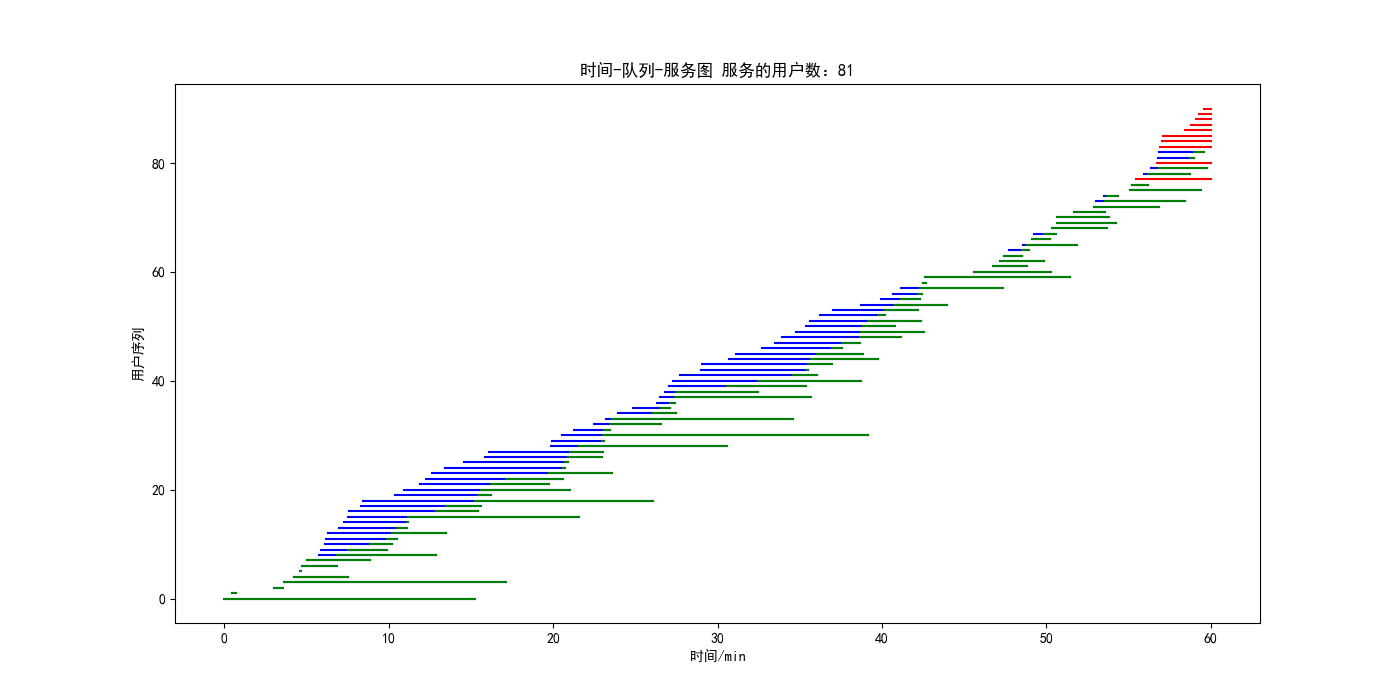
\includegraphics[width=0.35\textwidth]{figs/chap03/601.png}
%     }\subfigure[t=120]{\label{1201}
%     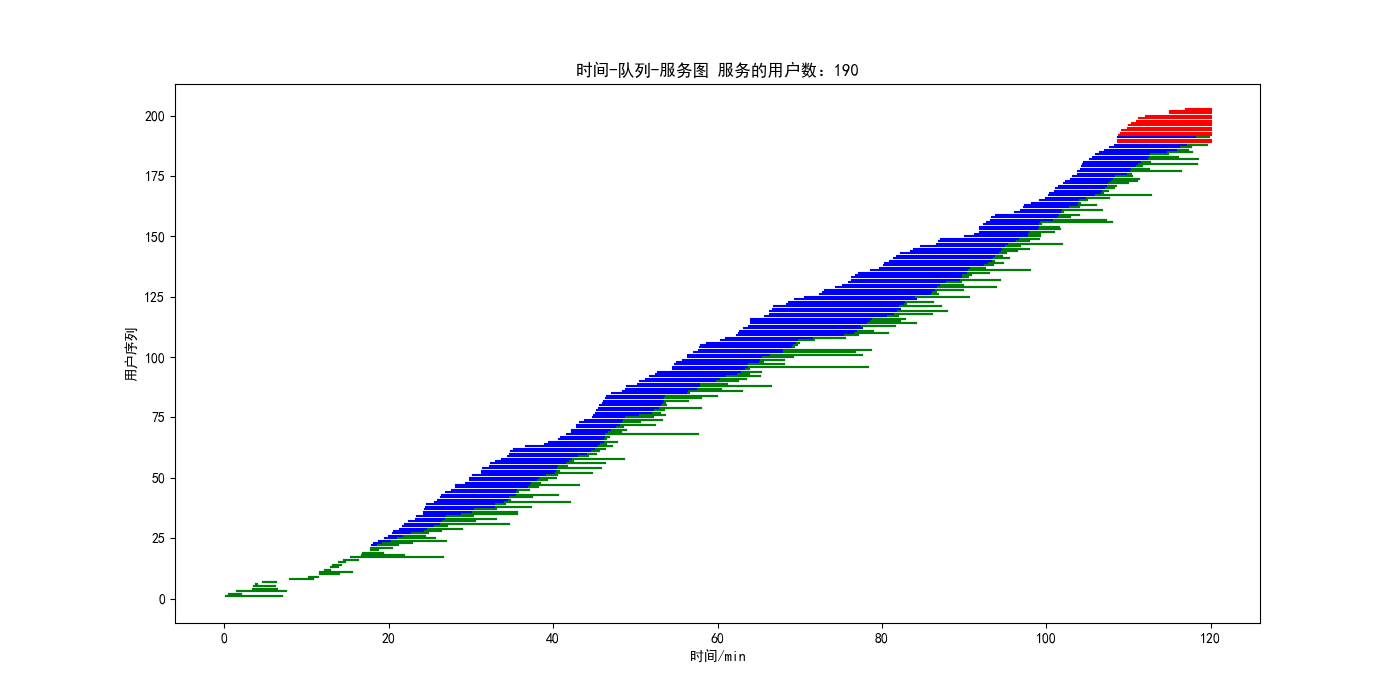
\includegraphics[width=0.35\textwidth]{figs/chap03/1201.png}
%     }
%     \\
%     \subfigure[t=180]{\label{1801}
%     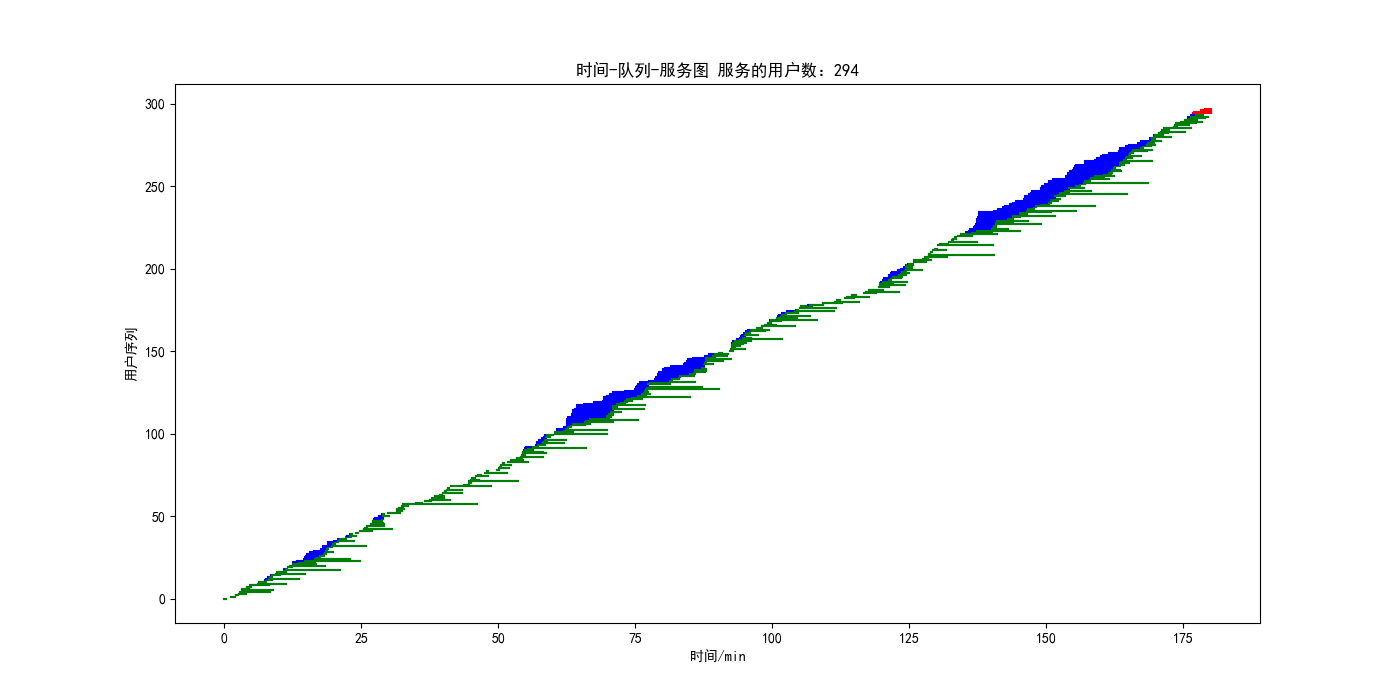
\includegraphics[width=0.35\textwidth]{figs/chap03/1801.png}
%     }\subfigure[t=240]{\label{2401}
%     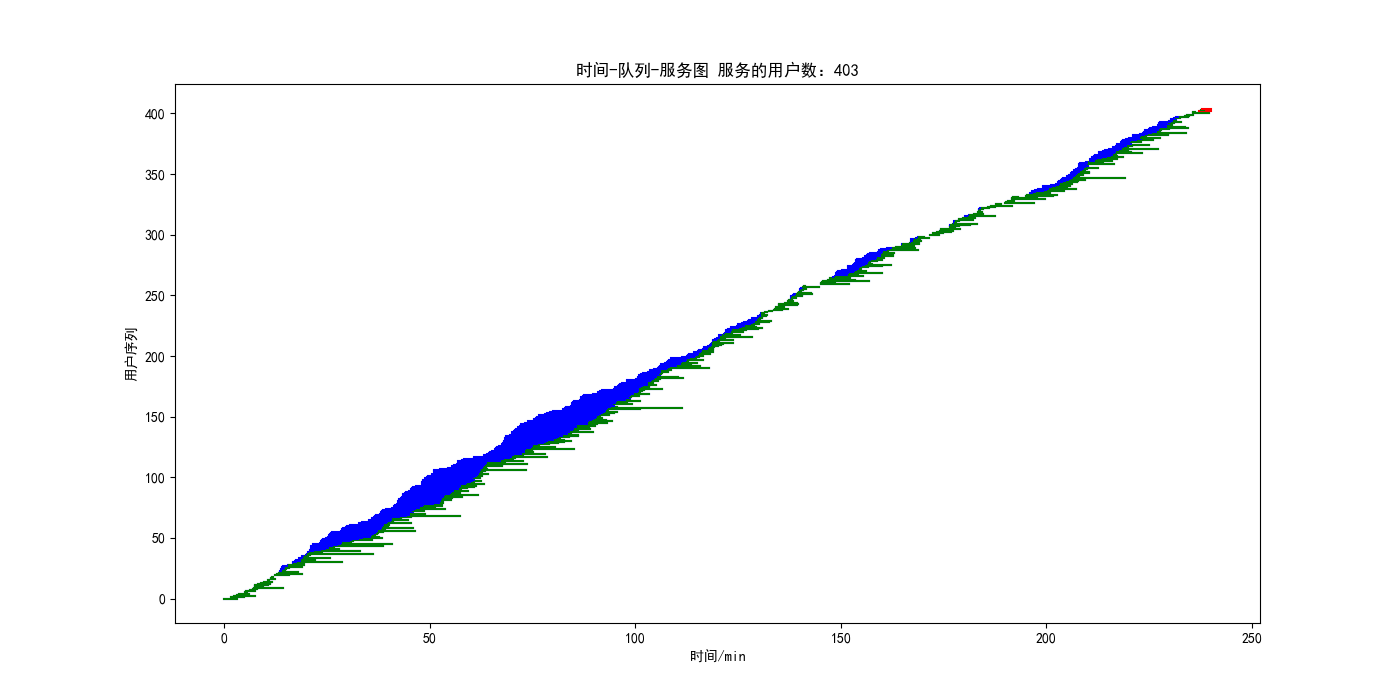
\includegraphics[width=0.35\textwidth]{figs/chap03/2401.png}
%     }
%     \caption{系统时间-队列-服务图}\label{fig34}
% \end{figure}

% 系统的时间-队列长度图:
% \begin{figure}[htbp]
%     \center
%     \subfigure[t=60]{\label{602}
%     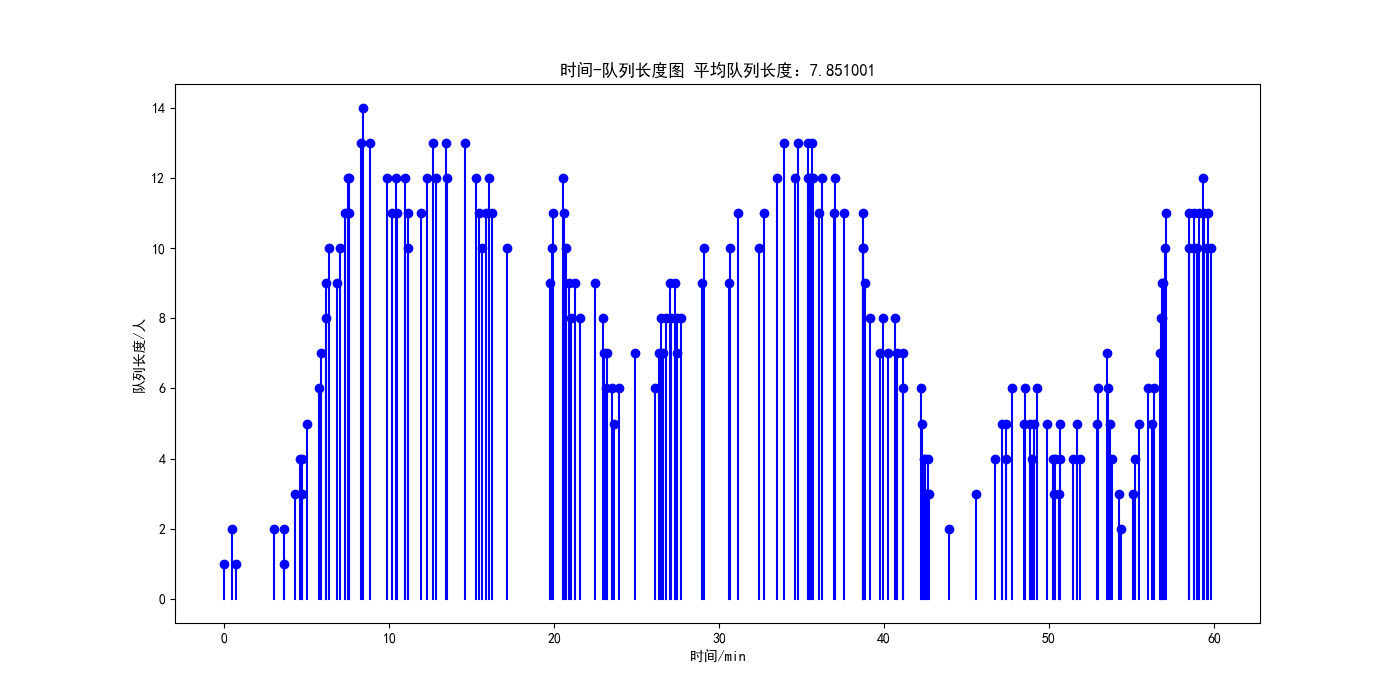
\includegraphics[width=0.45\textwidth]{figs/chap03/602.png}
%     }\subfigure[t=120]{\label{1202}
%     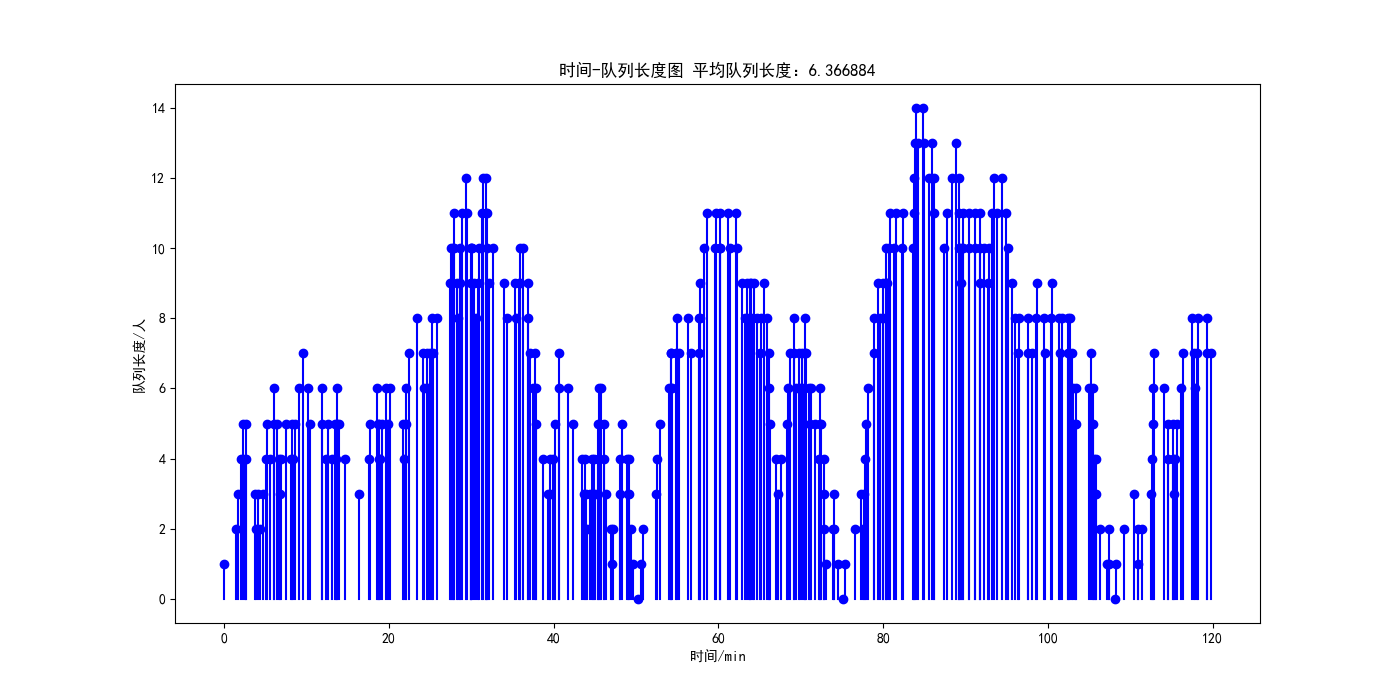
\includegraphics[width=0.45\textwidth]{figs/chap03/1202.png}
%     }
%     \\
%     \subfigure[t=180]{\label{1802}
%     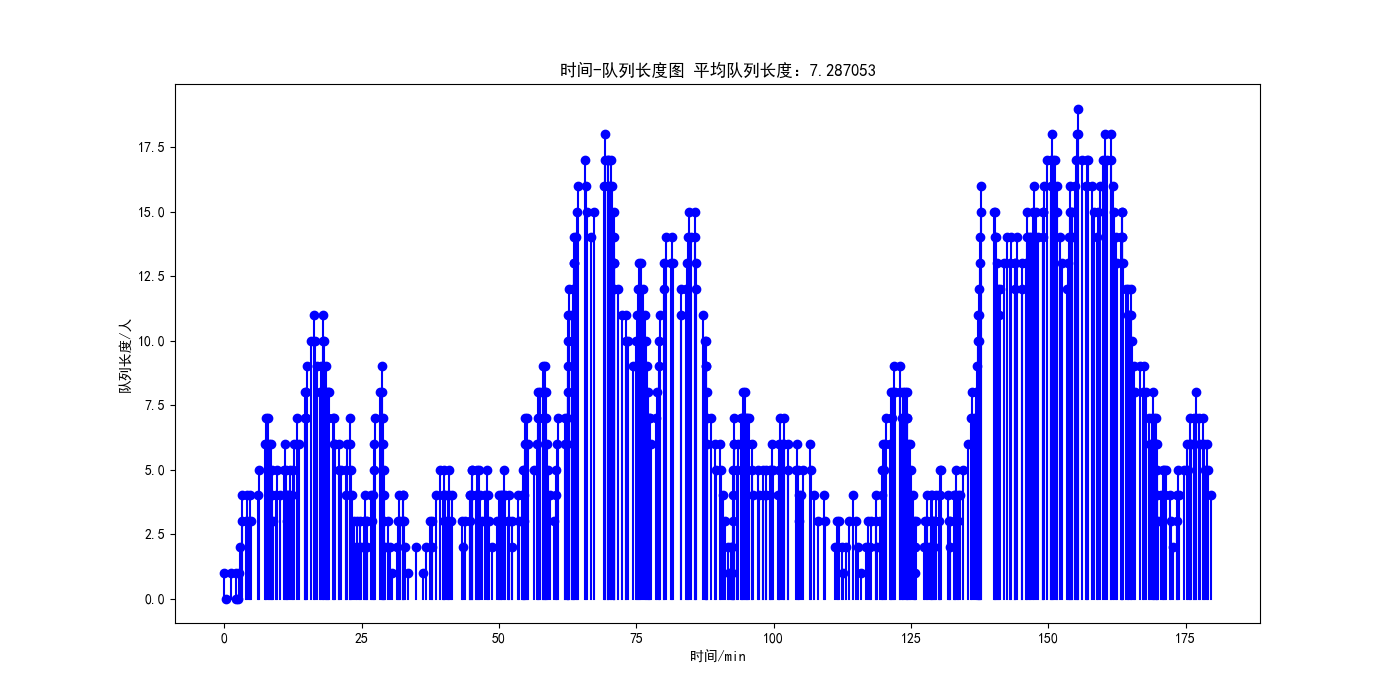
\includegraphics[width=0.45\textwidth]{figs/chap03/1802.png}
%     }\subfigure[t=240]{\label{2402}
%     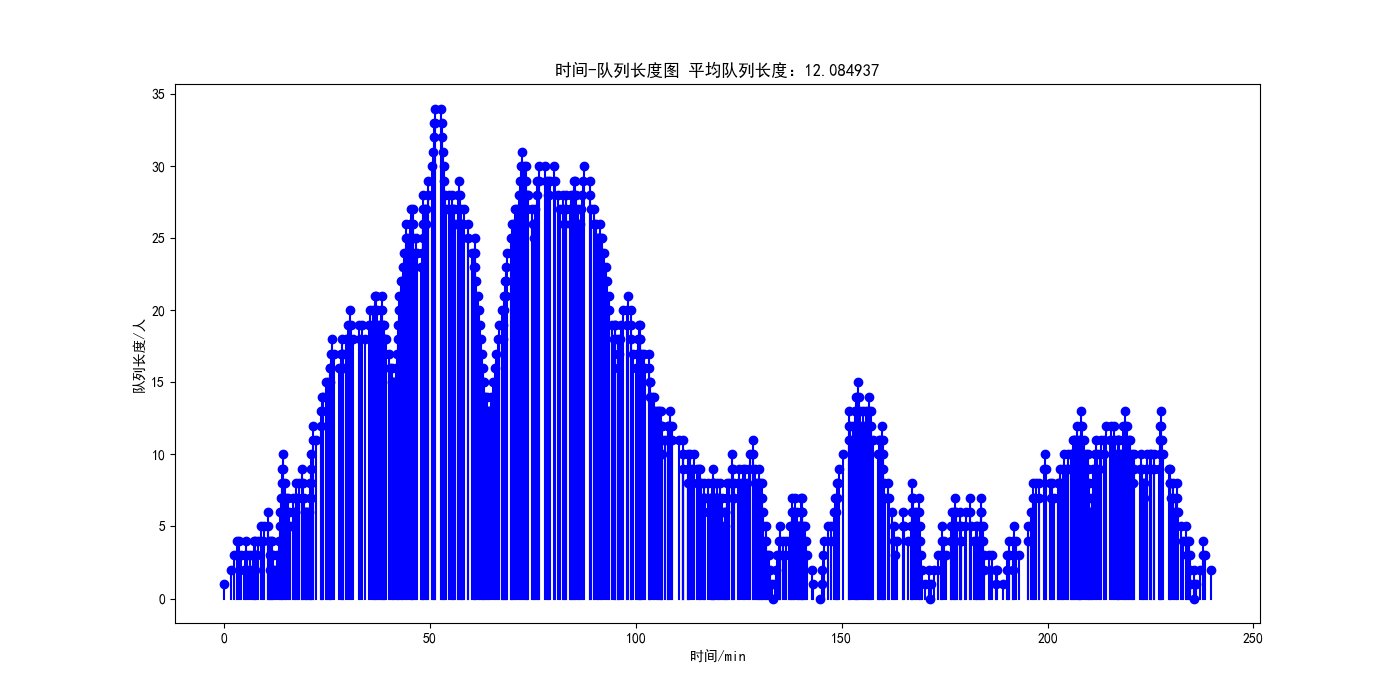
\includegraphics[width=0.45\textwidth]{figs/chap03/2402.png}
%     }
%     \caption{系统时间-队列长度图}\label{fig35}
% \end{figure}

% 系统的时间-等待时间图:
% \begin{figure}[htbp]
%     \center
%     \subfigure[t=60]{\label{603}
%     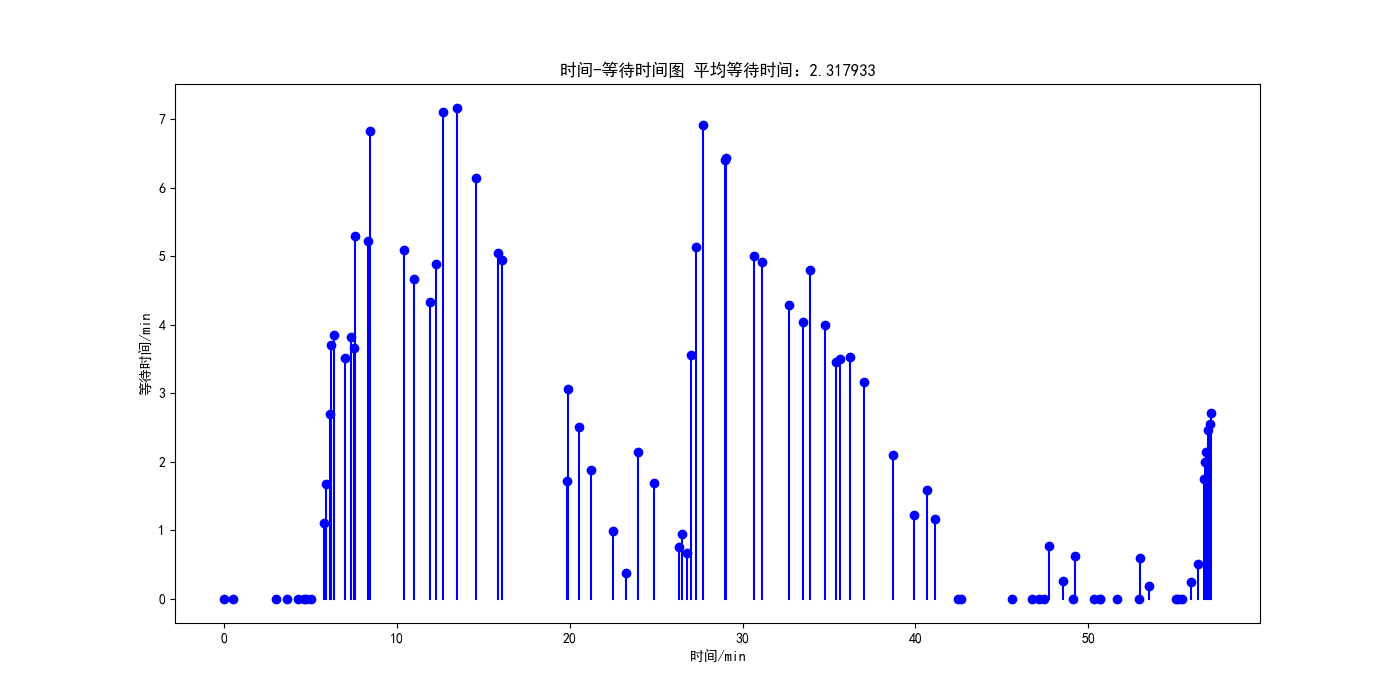
\includegraphics[width=0.43\textwidth]{figs/chap03/603.png}
%     }\subfigure[t=120]{\label{1203}
%     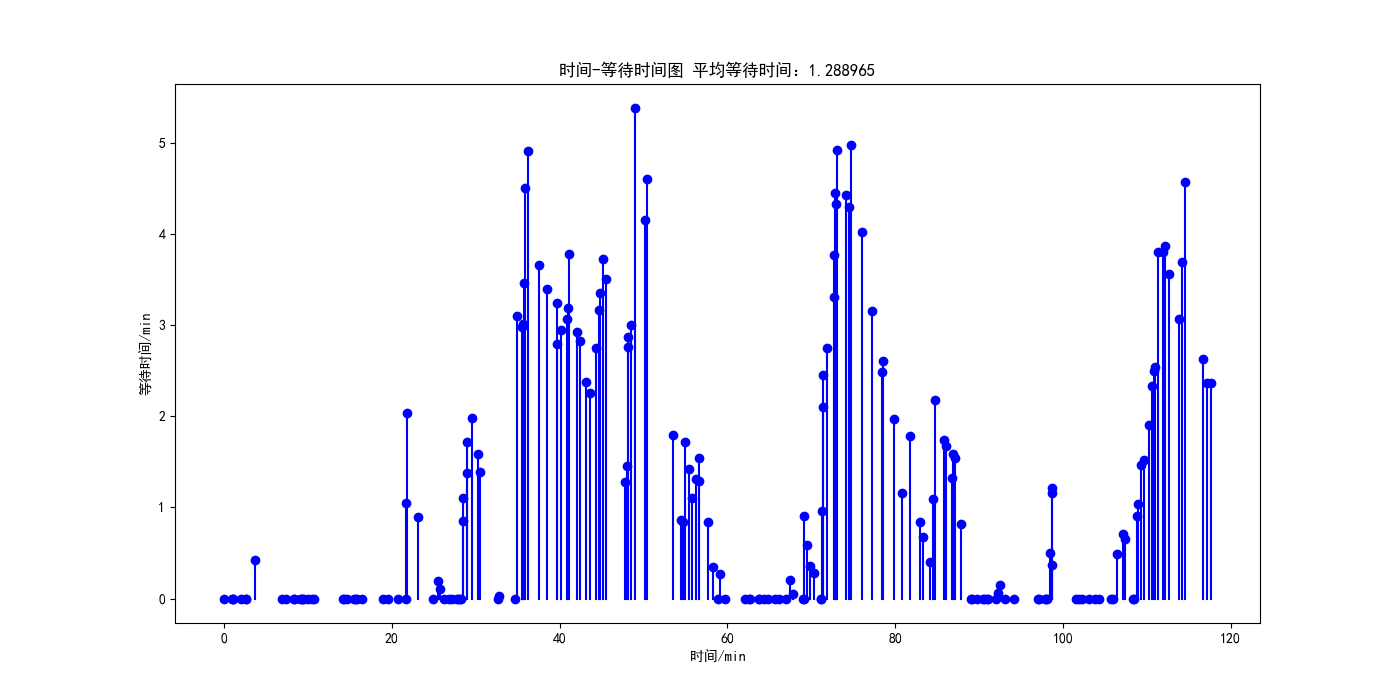
\includegraphics[width=0.43\textwidth]{figs/chap03/1203.png}
%     }
%     \\
%     \subfigure[t=180]{\label{1803}
%     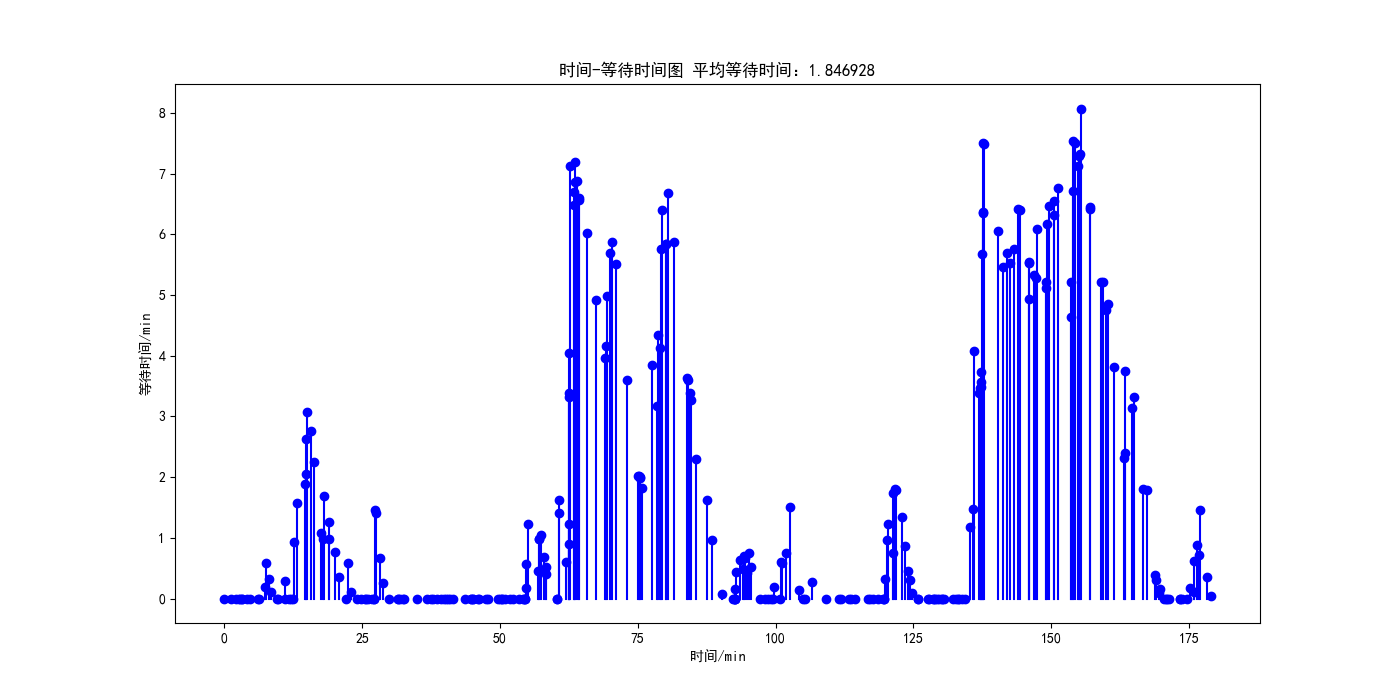
\includegraphics[width=0.43\textwidth]{figs/chap03/1803.png}
%     }\subfigure[t=240]{\label{2403}
%     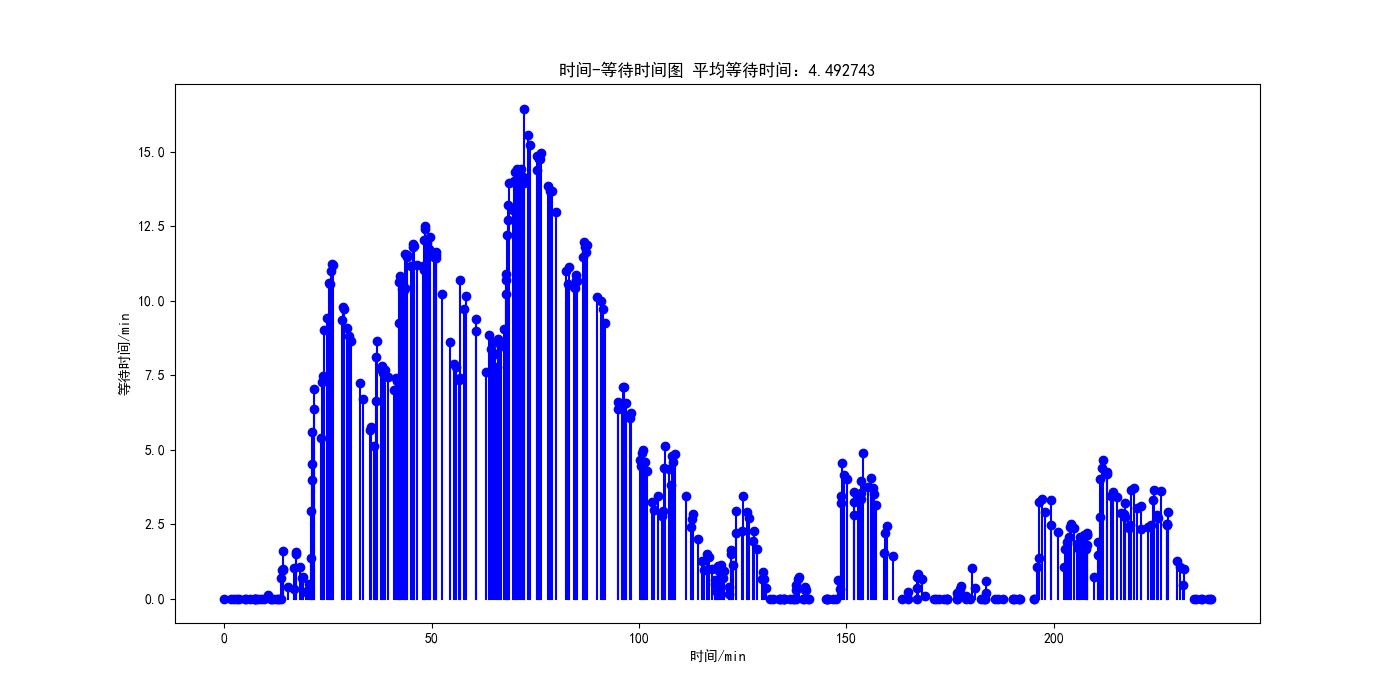
\includegraphics[width=0.43\textwidth]{figs/chap03/2403.png}
%     }
%     \caption{系统时间-等待时间图}\label{fig36}
% \end{figure}

\subsection{公交调度问题建模}
考虑单车型、多停车点、满载运输问题的一种启发式算法,并考虑使总空驶里程极
小为目标约束(对公交运营商的运输效益有极大影响)。

考虑一项货运业务,其发点为 $i'$,收点为 $i''$。假定有 $n$ 个可用的车站,
分别为 $A_{m+1}, \ldots, A_{m+n}$,可以发出和接收空车。每个车站可派出的空车数为 $b_j$,
可接收的空车数为 $b'_j$。该业务的货物量为 $g_i$,需要 $a_i$ 辆空车运输。
为使总空驶里程最小化,我们将该业务视为一个点,称为收缩点或重载点 $i$。
可以用网络中任意两点间的最短路径确定行车路线。
% 对于每个重载点 $i$,需要 $a_i$ 辆空车来运输货物 $g_i$。
% 这些车将在目的地卸货后提供 $a_i$ 辆空车,以继续执行运输任务。
% 设从点 $i$ 发往点 $j$($i, j$ 为车场或重载点)的空车数为 $x_{ij}$,其空驶里程为 $c_{ij}$。
空车调度问题的目标是使总空驶里程最小化,该问题可描述如下:
$$
\mathrm{T}:
\begin{cases}
    \min z=\sum_{i=1}^{m+n} \sum_{j=1}^{m+n} a_{j} x_{i j}\\
    \sum_{j=1}^{m+n} x_{i j}=a_{i}, \quad i=1,2, \cdots, m \\
    \sum_{j=1}^{m+n} x_{i j} \leqslant b, \quad i=m+1, m+2, \cdots, m+n \\
    \sum_{i=1}^{m+n} x_{i j}=a_{j}, \quad j=1,2, \cdots, m \\
    \sum_{i=1}^{m+n} x_{i j} \leqslant b_{j}, \quad j=m+1, m+2, \cdots, m+n\\
    x_{i j} \geqslant 0 \text { 且为整数 }
\end{cases}
$$
添加一个约束,这个约束的目标为使在车站的乘客等待时间最小。
在此基础上给出一个整数规划模型,这个模型给出具有线性约束。
这些约束联合同步每个车站的有效乘客装载时间窗口和车辆到达和离开时间。
以精确地制定来自不同O-D对的分钟依赖需求和小
时依赖需求量下的总等待时间。

考虑如何在路线的一个方向上设计需求响应时刻表,其中车站按顺序编号为 1;
2; ...; S,车辆服务从第一站移动到最后一站,如图~\ref{fig42}~。
\\
\begin{figure}[htbp]
    \centering
    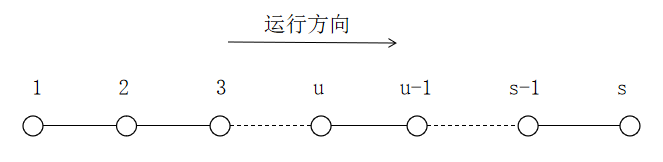
\includegraphics[width=0.8\textwidth]{figs/chap03/a.png}
    \caption{运行示意图}
    \label{fig42}
\end{figure}
\\

校园内公交线路共有10个车站,工作日每天有两个运行方向。
通过统计上下车的乘客数量,可以得到它们服从的分布函数。
假设该线路上运行的所有车辆都有相同的运力,标准载客量为22人。
该线路的平均速度为15公里/小时。
为了保证成本效益和用户体验,有以下约束条件:
一般情况下,乘客在车站等待的时间不应该大于十分钟;同时给出一个硬性约束车辆荷载人数不能超过22人。
同时为了节约公交的运营成本,车辆的运营时期车上的空座位数量应该尽量不大于一半。

% 该调度问题可以抽象为两个子问题:

% (1) 建立模拟公交车运营的运行模型,即确定在某一调度方案下,公交车在该线路上运行的数学描述。一种比较实际的方法是采用随机模型,通过随机模拟来模拟运行过程,使用决策变量和原始数据计算出各种目标数值。另一种是建立确定性模型,将运行过程看作是按照一定时间表发车的公交车,在一定要求下按照预定的顺序将沿线乘客送达预定地点的确定过程。

% (2) 通过运行模型来优化目标。本问题实际上是一个多目标规划问题,至少有两个目标需要考虑:一个是反映乘客利益的乘客等待时间;另一个是反映公交运营成本的载客率。

算法中出现的参数描述和相关计算公式如下:
\begin{table}[htbp!]
    \centering
    \caption{参数表}\label{teble_3}
    \begin{tabular}{cc}
        \whline
        参数 & 参数含义 \\
        \hline
        j=1,2,……,n & 车站标志\\
        $P_j(t) \sim \frac{\lambda^t}{t!}e^{-\lambda},j=1,2,…,n$ & 客流密度(t时刻到达j车站的乘客密度)\\
        $\tau_j,j=1,2,…,n$ & 车站间行车时间(从j到j+1站的行车时间)\\
        $d_j{j}$ & 第j站的下车人数\\
        B & 载客容量 \\
        $\hat{B}$ & 容量上限\\
        $\widehat{t}$ &  高峰期乘客等待时间上限 \\
        $\hat{t}$ & 平峰时段乘客等待时间上限 \\
        $t = (T_0,T_1,T_2,…,T_k,…,T_m)$ & 决策变量(发车时刻表)\\
        $T_{k1} = T_k, T_{kj} = T_{k1} + \sum_{\ell = 1}^{j-1}, j = 1, 2, 3, …,n-1$ & 第k班次驶离j站的时刻 \\
        $D_k(T_{kj})$ & 第k辆车驶离j站时该车上的乘客数\\
        \whline
    \end{tabular}
\end{table}


(1)第k辆车到达j站后,车上剩余乘客数:
$$
a_{kj} = max{(D_k(T_{kj-1}) - \int\limits_{T_{k-1}}^{T_{kj}}d_j(t)dt ), 0};
$$

(2)第k辆车驶到j站后可容纳的上车乘客数上界 :
$$
b_{kj} = \hat{b} - a_{kj};
$$

(3)第k - 1辆车驶离j站到第k辆车驶到j站时段内,到达的乘客数量:
$$
W_{kj}(0) = \int\limits_{T_{kj}}^{K_{k-1}}P_j(t)dt;
$$

求出可行解 $T = (T_0,T_1,t_2,…T_k,…,T_m)$符合目标函数:
$$
min C = W_1(T)d_1+W_2(T)d_2 + low(T)d_3
$$

在每个车站按FIFO(先来先服务)原则提供服务,在第k+1号车到达j个站台
时,需要的车辆最大值 $h_{kj}^*$ 符合如下规划问题:
$$
\underset{0 \le h \le h_{kj}}{max} h  
$$
$$
\sum_{r=h}^{h_{kj}}W_{kj}(r) \le b_{kj}
$$

% 该算法计算框图如图~\ref{11}~
% \begin{figure}[htbp!]
%     \center
%     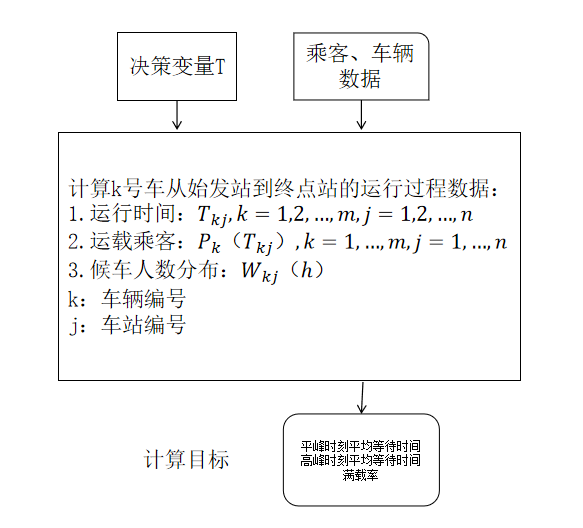
\includegraphics[width=0.9\textwidth]{figs/chap03/k.png}
%     \caption{算法计算框图}
%     \label{11}
% \end{figure}

使用GurboiPy建立该问题的模型,核心代码如下:
\begin{lstlisting}[breaklines=true,language=Python]
    class MyModel():
    def __init__(self):
        self.model = gp.Model()
        self.m = 3
        self.n = 4
        for i in range(self.m):
            for j in range(self.n):
                self.cij[(i, j)] = self.table_value[i][j][0]
                self.dij[(i, j)] = self.table_value[i][j][1]

    def define_decision_var(self):
        self.xij = gp.tupledict()
        for i in range(self.m):
            for j in range(self.n):
                self.xij[i,j] = self.model.addVar(vtype=gp.GRB.INTEGER)

    def add_basic_cos(self):
        for i in range(self.m):
            cos1 = 0
            for j in range(self.n):
                cos1 += self.xij[i, j]
            self.model.addConstr(cos1 == self.a[i])
        for j in range(self.n):
            cos2 = 0
            for i in range(self.m):
                cos2 += self.xij[i, j]
            self.model.addConstr(cos2== self.b[j])

    def add_new_cos(self, cos_left, cos_right):
        self.model.addConstr(cos_left == cos_right)
\end{lstlisting}

该算法计算框图如图~\ref{11}~
\begin{figure}[htbp!]
    \center
    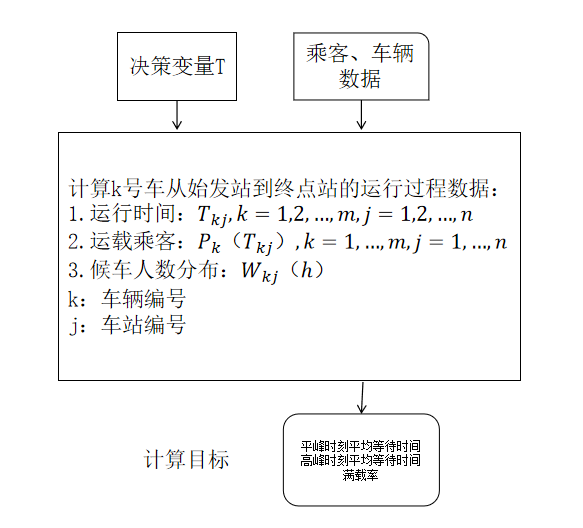
\includegraphics[width=0.7\textwidth]{figs/chap03/k.png}
    \caption{算法计算框图}
    \label{11}
\end{figure}
